% -*- latex -*-
%%%%%%%%%%%%%%%%%%%%%%%%%%%%%%%%%%%%%%%%%%%%%%%%%%%%%%%%%%%%%%%%
%%%%
%%%% This TeX file is part of the course
%%%% Introduction to Scientific Programming in C++/Fortran2003
%%%% copyright 2017-2023 Victor Eijkhout eijkhout@tacc.utexas.edu
%%%%
%%%% array.tex : basic language elements
%%%%
%%%%%%%%%%%%%%%%%%%%%%%%%%%%%%%%%%%%%%%%%%%%%%%%%%%%%%%%%%%%%%%%

An \indextermdef{array}\footnote
{The term `array' is used informally here.
  There is an \texttt{array} keyword,
  which is briefly discussed in section~\ref{sec:cpp-array}.}
is an indexed data structure that for each
index stores an integer, floating point number, character,
object, et cetera.
In scientific applications, arrays often correspond to vectors and
matrices, potentially of quite large size. (If you know about the
\acf{FEM}, you know that vectors can have sizes in the millions or beyond.)

In this chapter you will see the C++ \indexc{vector} construct,
which implements the notion of an array of things, whether they be
numbers, strings, objects.

\begin{slide}{What are vectors?}
  \label{sl:what-vector}
  \begin{itemize}
  \item Contiguous, indexed, storage of items:\\
    (often called `array' but that has other meanings)
    \begin{itemize}
    \item items of any type (but the same for all elements of one
      vector)
    \item potentially very many items
    \end{itemize}
  \item Indexed set of items
  \item \ldots~but if you don't need the index: collection of items
  \end{itemize}
\end{slide}

\begin{cnote}
  While C++ can use the C~mechanisms for arrays, for almost all purposes
  it is better to use \lstinline{vector}. In particular, this is a safer way to
  do dynamic allocation. The old
  mechanisms are briefly discussed in section~\ref{sec:staticarray}.
\end{cnote}

\begin{slide}{C++ Vectors are better than C arrays}
  \label{sl:vector-why}
  Vectors are fancy arrays. They are easier and safer to use:
  \begin{itemize}
  \item They know what their size is.
  \item Bound checking.
  \item Freed when going out of scope: no memory leaks.
  \item Dynamically resizable.
  \end{itemize}
  In C++ you never have to \indexc{malloc} again.\\
  (Not even \indexc{new}.)
\end{slide}

\Level 0 {Some simple examples}

\Level 1 {Vector creation}

To use vectors, you first need the \indexheader{vector} header from the \ac{STL}.
This allows you to declare a vector, specifying what type of element
it contains. Next you may want to decide how many elements it
contains; you can specify this when you declare the vector, or
determine it later, dynamically.

We start with the most obvious way of creating a vector:
enumerating its elements.

\begin{block}{Short vectors}
  \label{sl:vectorshort}
  Short vectors can be created by enumerating their elements:
  %
  \lstset{style=snippetcode}
  \verbatimsnippet{shortvectorex}
\end{block}

\begin{exercise}
  \label{ex:shortvectoralter}
  \begin{enumerate}
  \item
    Take the above snippet, compile, run.
  \item Add a statement that alters the value of a vector element.
    Check that it does what you think it does.
  \item Add a vector of the same length as the \lstinline{evens} vector,
    containing odd numbers
    which are the even values plus~1?
  \end{enumerate}
  \skeleton{shortvector}
\end{exercise}

For a less simple example, let's make a \lstinline{vector}
containing objects, in this case the \lstinline{Point} objects:
\begin{lstlisting}
vector<Point> diagonal = 
    { {0.,0.}, {1.,1.}, {1.5,1.5}, {2.,2.}, {3.,3.} };
\end{lstlisting}

\Level 1 {Initialization}

There are various ways to declare a vector, and possibly initialize it.

More generally, vectors can be defined
\begin{itemize}
\item Without further specification, creating an empty vector:
\begin{lstlisting}
vector<float> some_numbers;
\end{lstlisting}
\item With a size indicated, allocating that number of elements:
\begin{lstlisting}
vector<float> five_numbers(5);
\end{lstlisting}
(This sets the elements to a default value; zero for numeric types.)
\item You can initialize a vector with a constant:
\begin{lstlisting}
vector<float> x(25,3.15);
\end{lstlisting}
which defines a vector \lstinline{x} of size~25,
with all elements initialized to~3.15.
\end{itemize}

\begin{slide}{Vector constant initialization}
  \label{sl:vector-initconst}
  There is a syntax for initializing a vector with a constant:
\begin{lstlisting}
vector<float> x(25,3.15);
\end{lstlisting}
which defines a vector \lstinline{x} of size~25,
with all elements initialized to~3.15.
\end{slide}

If your vector is short enough, you can set all elements explicitly with an
\indextermbus{initializer}{list}, as you saw above.
Note that the size is not specified here,
but is deduced from the length of the initializer list:

\snippetwithoutput{dynamicinit}{array}{dynamicinit}

\begin{slide}{Vector initialization}
  \label{sl:vector-init}
  You can initialize a vector as a whole:
  \begin{lstlisting}
    vector<float> halves{ 0.5, 1.5, 2.5, 3.5 };
  \end{lstlisting}
  (Note: no size given)
\end{slide}

\begin{slide}{Vector definition}
  \label{sl:vector-def}
  Definition and/or initialization:
  \lstset{style=snippetcode}
\begin{lstlisting}
#include <vector>
using std::vector;

vector<type> name;
vector<type> name(size);
vector<type> name(size,init_value);
\end{lstlisting}
where
\begin{itemize}
\item \indexc{vector} is a keyword,
\item \n{type} (in angle brackets) is any elementary type or class
  name,
\item \n{name} of the vector is up to you, and
\item \n{size} is the (initial size of the vector). This is an integer,
  or more precisely, a \indexc{size_t} parameter.
\item Initialize all elements to \n{init_value}.
\item If no default given, zero is used for numeric types.
\end{itemize}
\end{slide}

\begin{review}
  T/F? 
  \begin{itemize}
  \item It is possible to write a valid C++ program where you define a
    variable \lstinline+vector+.
  \end{itemize}
\end{review}

\Level 1 {Element access}

There are two ways of accessing vector elements.
\begin{enumerate}
\item With the `dot' notation that you know from structures and objects, 
  you can use the \indexc{at} method:
  \snippetwithoutput{assignatfun}{array}{assignatfun}
  The expression \lstinline+a.at(i)+ can be used to get the value of a
  vector element, or it can occur in the left-hand side of an
  assignment to set the value.
\item
  There is also a short-hand notation (which is the same as in~C):
\snippetwithoutput{assignbracket}{array}{assignbracket}
  Again, the element accessed can be used both in left and right hand sides.
\end{enumerate}

Indexing starts at zero. Consequently, a vector declared as
\begin{lstlisting}
vector<int> ints(N)
\end{lstlisting}
has elements $0,\ldots,N-1$.

\begin{slide}{Accessing vector elements}
  \label{sl:vectorsub}
  Square bracket notation (zero-based):
  \snippetwithoutput{assignbracket}{array}{assignbracket}

  With bound checking:
  \snippetwithoutput{assignatfun}{array}{assignatfun}
  Safer, slower.\\
  (Remember Knuth about optimization.)
\end{slide}

\Level 1 {Access out of bounds}

Have you wondered what happens if you access a
vector element outside the bounds of the vector?
\begin{lstlisting}
vector<float> x(6); // size 6, index ranges 0..5
x.at(6) = 5.; // oops!
i = -2;
x[i] = 3; // also oops, but different.
\end{lstlisting}
Often it is hard for the compiler to determine that you are
accessing an element outside the vector bounds.
Most likely, it will only be detected at runtime.
There is now a difference in how the two accessing methods
do \indextermbus{vector}{bounds checking}.

\begin{slide}{Vector elements out of bounds}
  \label{sl:vectorsuboob}
  Square bracket notation:
  \snippetwithoutput{assignbracketoob}{array}{assignoutofboundbracket}

  With bound checking:
  \snippetwithoutput{assignatfunoob}{array}{assignoutofboundatfun}
  Safer, slower.\\
  (Remember Knuth about optimization.)
\end{slide}

\begin{enumerate}
\item Using the \indexc{at} method will always do a bounds test,
  and exit your program immediately if you access an element
  outside the vector bounds.
  (Technically, it throws an \indexterm{exception};
  see section~\ref{sec:exception} for how this works and how you can handle this.)
\item The bracket notation \lstinline{a[i]} performs no bounds tests:
  it calculates a memory address based on the vector location and the index,
  and attempts to return what is there.
  As you may imagine, this lack of checking makes your code a little faster.
  However, it also makes your code unsafe:
  \begin{itemize}
  \item Your program may crash with a \indexterm{segmentation fault}
    or \indexterm{bus error}, but no clear indication where and why this happened.
    (Such a crash can be caused by other things than vector access out of bounds.)
  \item Your program may continue running, but  giving wrong results,
    since reading from outside the vector probably gives you meaningless values.
    Writing outside the bounds of an vector may even change the data of other variables,
    leading to really strange errors.
  \end{itemize}
\end{enumerate}
For now, it is best to use the \indexc{at} method throughout.

\begin{block}{Vector index out of bounds}
  Indexing out of bounds can go undetected for a while:
  
  \snippetwithoutput{vectoroutofbound}{array}{segmentation}
\end{block}

\begin{review}
  The following codes are not correct in some sense. How will this manifest itself?
  %\verbatimsnippet{staterr}
  \verbatimsnippet{vecerr}
  \verbatimsnippet{vecexc}
\end{review}

\Level 0 {Going over all vector elements}
\label{sec:arrayrange}

If you need to consider all the elements in a vector, you typically
use a \indexc{for} loop. There are various ways of doing this.

\begin{block}{A philosophical point}
  \label{sl:vector-access-types}

  Conceptually, a \indexc{vector} can correspond to a set of things,
  and the fact that they are indexed is purely incidental,
  or it can correspond to an ordered set,
  and the index is essential.
  If your algorithm requires you to access all elements,
  it is important to think about which of these cases apply,
  since there are two different mechanism.
\end{block}

\Level 1 {Ranging over a vector}

First of all consider the cases where you consider the vector as a
collection of elements, and the loop functions like a mathematical
`for all'.
This uses a `colon' notation.

\index{range-based for loop|see{for, range-based}}
\begin{block}{Range over elements}
  \label{sl:vector-range1}
  A \indextermsub{range-based}{for} loop
  gives you directly the element values:
\begin{lstlisting}
vector<float> my_data(N);
/* set the elements somehow */;
for ( float e : my_data )
  // statement about element e
\end{lstlisting}
Here there are no indices because you don't need them.
\end{block}

You can spell out the type of the vector element, but such type
specifications can be complex.
In that case, using \indextermbus{type}{deduction}
through the \indexc{auto} keyword
is quite convenient.

\begin{block}{Range over elements, version 2}
  \label{sl:vector-range2}
  Same with \indexc{auto} instead of
  an explicit type for the elements:
\begin{lstlisting}
for ( auto e : my_data )
  // same, with type deduced by compiler
\end{lstlisting}
\end{block}

As an example, consider finding the maximum value
in an array of numbers.
Since we only want the value, not where it is placed,
we use this range-based syntax.
(Note: there is actually a library function for this,
so this example is mostly for the sake of discussing the ranging mechanism.)

\begin{block}{Range over elements}
  \label{sl:vector-range3}
  Finding the maximum element
  \snippetwithoutput{dynamicmax}{array}{dynamicmax}
\end{block}

Another note: the initialization to a large negative value
can be done more elegantly; see section~\ref{sec:limits}.

So-called \indextermbus{initializer}{list}s
can also be used as a list denotation:

\begin{block}{Range over vector denotation}
  \label{sl:range-denote}
  \snippetwithoutput{rangedenote}{array}{rangedenote}  
\end{block}

\Level 1 {Ranging over the indices}

If you actually need the index of the element, you can use a
traditional \indexc{for} loop with loop variable.

\begin{block}{Indexing the elements}
  \label{sl:index-range}
  You can write an \indextermsub{indexed}{for} loop, which uses an
  index variable that ranges from the first to the last element.
\begin{lstlisting}
for (int i= /* from first to last index */ )
  // statement about index i
\end{lstlisting}
Example: find the maximum element in the vector, and where it occurs.
%
\renewcommand\snippetcodefraction{.67}
\renewcommand\snippetanswfraction{.3}
\snippetwithoutput{vecidxmax}{array}{vecidxmax}
\end{block}

\begin{exercise}
  \label{ex:range-for}
  Indicate for each of the following vector operations whether you
  prefer to use an indexed loop or a range-based loop. Give a short
  motivation.
  \begin{itemize}
  \item Count how many elements of a vector are zero.
  \item Find the location of the last zero.
  \end{itemize}
\end{exercise}

\begin{exercise}
  \label{ex:array-max}
  Find the element with maximum absolute value in a vector. Use:
\begin{lstlisting}
vector<int> numbers = {1,-4,2,-6,5};
\end{lstlisting}
% Which mechanism do you use for traversing the vector?

Hint:
\begin{lstlisting}
#include <cmath>
..
absx = abs(x);
\end{lstlisting}
\end{exercise}

\begin{exercise}
  \label{ex:array-maxidx}
  Find the location of the first negative element in a vector.

  Which mechanism do you use?
\end{exercise}

\begin{exercise}
  \label{ex:array-sorted}
  Check whether a vector is sorted.
\end{exercise}

\Level 1 {Ranging by reference}

In the previous examples we only read out the values
of the vector elememts.
What if you want to access the element values in order to  change them,
for instance to add something to them, or multiply them?

Range-based loops can do this.
You need to realize that in the loops so far
\begin{lstlisting}
for ( auto e : my_array )
  // something with e  
\end{lstlisting}
the variable \lstinline{e} actually contains a copy of the vector elements.
This means that altering \lstinline{e} does not affect the vector.
To get that effect, you need to make \lstinline{e} a reference to the vector elements.

\begin{lstlisting}
for ( auto &e : my_vector)
  e = ....
\end{lstlisting}

\begin{slide}{Range over elements by reference}
  \label{sl:vector-range-ref}
  Range-based loop indexing makes a copy of the vector element. If you
  want to alter the vector, use a reference:
  %
\begin{lstlisting}
for ( auto &e : my_vector)
  e = ....
\end{lstlisting}
%
\snippetwithoutput{vectorrangeref}{array}{vectorrangeref}

(Can also use \lstinline{const auto& e} to prevent copying, but also
prevent altering data.)
\end{slide}

\begin{block}{Example: multiplying elements}
  \label{sl:range-ref-ex}
Example: multiply all elements by two:
\snippetwithoutput{vectorrangeref}{array}{vectorrangeref}
\end{block}

\begin{exercise}
  If you do the prime numbers project, you can now do exercise~\ref{ex:arraysieve}.
\end{exercise}

\Level 1 {Arrays and while loops}

In a \indexc{while} loop, if you need an index,
you need to maintain that index explicitly.
There are then certain common idioms.

\begin{block}{Example of increment indexing}
  \label{sl:plusplusexample}
  \snippetwithoutput{plusplustest1}{loop}{plusplus}
\end{block}

\begin{slide}{Indexing with pre/post increment}
  \label{sl:prepostindex}
Indexing in \indexc{while} loop and such:
\begin{lstlisting}
x = a.at(i++); /* is */ x = a.at(i); i++;
y = b.at(++i); /* is */ i++; y = b.at(i);
\end{lstlisting}
\end{slide}

\begin{exercise}
  Exercise: modify the preceding code so that after the while loop
  \n{index} is the number of leading odd elements.
\end{exercise}

\Level 0 {Vector are a class}
\label{sec:stdvector}

Above, you created vectors and used functions \indexc{at} and \indexc{size}
on them. They used the dot-notation of class methods, and in fact
vector form a \indexcdef{vector} class. You can have a vector of ints,
floats, doubles, et cetera; 
the angle bracket notation indicates what the specific type stored in
the vector is.
You could say that the vector class is parameterized with the type (see
chapter~\ref{ch:template} for the details).
You could also say that
\lstinline{vector<int>} is a new data type,
pronounced `vector-of-int', and you can
make variables of that type.

\begin{slide}{Your first encounter with templates}
  \label{sl:vector-template}
 \lstinline{vector} is a `templated class':
    \lstinline{vector<X>} is a vector-of-\lstinline{X}.

    Code behaves as if there is a class definition for each type:
    \begin{multicols}{2}
      \small
\begin{lstlisting}
class vector<int> {
public:
  size(); at(); // stuff
}
\end{lstlisting}
\begin{lstlisting}
class vector<float> {
public:
  size(); at(); // stuff
}
\end{lstlisting}
    \end{multicols}
    Actual mechanism uses templating:
    the type is a parameter to the class definition.
\end{slide}

\begin{block}{Vector copy}
  \label{sl:vectorcopy}
  Vectors can be copied just like other datatypes:
  %
  \snippetwithoutput{vectorcopy}{array}{vectorcopy}
  %
\begin{cpp4c}
    Note: contents copied, not just pointer.
\end{cpp4c}
\end{block}

\Level 1 {Vector methods}

There are several \emph{methods}\index{vector!methods}
to the \lstinline{vector} class. Some of the simpler ones are:
\begin{itemize}
\item \indexc{at}: index an element
\item \indexc{size}: give the size of the vector
\item \indexc{front}: value of the first element
\item \indexc{back}: value of the last element
\end{itemize}

There are also methods relating to dynamic storage management, which
we will get to next.

\begin{exercise}
  \label{ex:vectornormalize}
  Create a \n{vector} $x$ of \lstinline{float} elements, and set them to random
  values. (Use the C random number generator for now.)

  Now normalize the vector in $L_2$ norm and check the correctness of
  your calculation, that is,
  \begin{enumerate}
  \item Compute the $L_2$ norm of the vector:
    \[ \| v\| \equiv \sqrt{\sum_iv_i^2} \]
  \item Divide each element by that norm;
  \item The norm of the scaled vector should now by~1. Check this.
  \item Bonus: your program may be printing~1, but is it actually~1?
    Investigate.
  \end{enumerate}
  What type of loop are you using?
\end{exercise}


\begin{slide}{Vector methods}
  \label{sl:vector-method}
  A vector is an object, with methods.

  Given \lstinline+vector<sometype> x+:
  \begin{itemize}
  \item Get elements, including bound checking, with
    \lstinline{ar.at(3)}.
    Note: (zero-based indexing).
  \item (also get elements with \lstinline{ar[3]}: see later discussion.)
    %% (for C programmers: this is not dereferencing, this uses an
    %% operator method)
  \item Size: \lstinline{ar.size()}.
  \item Other functions: \indexc{front}, \indexc{back}, \indexc{empty}.
  \item With iterators (see later): \indexc{insert}, \indexc{erase}
  \end{itemize}
\end{slide}

\Level 1 {Vectors are dynamic}
\label{sec:stdvector-dynamic}

A vector
can be grown or shrunk after its creation.
For instance, you can use the \indexc{push_back} method to add elements at the end.

\begin{block}{Dynamic vector extension}
  \label{sl:vector-dynamic}
  Extend a vector's size with \indexc{push_back}:
  %
  \snippetwithoutput{vectorpush}{array}{vectorend}
  %
  Similar functions: \indexc{pop_back}, \indexc{insert}, \indexc{erase}.
  \slidenewline
  Flexibility comes with a price.
\end{block}

It is tempting to use \indexc{push_back} to create a vector dynamically.

\begin{block}{When to push back and when not}
  \label{sl:vecpushnot}
  \begin{multicols}{2}
    Known vector size:
\begin{lstlisting}
int n = get_inputsize();
vector<float> data(n);
for ( int i=0; i<n; i++ ) {
  auto x = get_item(i);
  data.at(i) = x;
}
\end{lstlisting}
\columnbreak
    Unknown vector size:
\begin{lstlisting}
vector<float> data;
float x;
while ( next_item(x) ) {
  data.push_back(x);
}
\end{lstlisting}
  \end{multicols}
  If you have a guess as to size: \lstinline+data.reserve(n)+.

  (Issue with array-of-object: in left code, constructors are called twice.)
\end{block}

\begin{block}{Dynamic size extending}
  \label{sl:vector-extend}
\begin{lstlisting}
vector<int> iarray;
\end{lstlisting}
creates a vector of size zero. You can then
\begin{lstlisting}
iarray.push_back(5);
iarray.push_back(32);
iarray.push_back(4);
\end{lstlisting}
\end{block}

However, this dynamic resizing involves memory management, and maybe
operating system functions. This will probably be
inefficient. Therefore you should use such dynamic mechanisms only
when strictly necessary.
If you know the size,
create a vector with that size. If the size is not precisely known but
you have a reasonable upper bound, you can call \indexc{reserve} to
reserve space for that many elements:
\begin{lstlisting}
vector<int> iarray;
iarray.reserve(100);
while ( ... )
  iarray.push_back( ... );
\end{lstlisting}

The combination of using \indexc{reserve} and \indexc{push_back}
can be preferable over creating the vector immediately with a certain size.
Writing \lstinline+vector<X> xs(100)+, where \lstinline{X} is some object,
causes the default constructor of~\lstinline{X} to be called on each vector element.
For complicated objects this may not be advisable.

\Level 0 {The Array class}
%%packtsnippet stdarray
\label{sec:cpp-array}
\label{sec:stdarray}

In cases where an array will never change size it would be convenient
to have a variant of the \lstinline{vector} class that does not have
the dynamic memory management facility.
The \indexcdef{array} class seems to fulfill this role at first sight.
However, it
is limited to arrays where the size is known at compile time,
so you can not for instance read it in as a parameter.

\verbatimsnippet{incstdarray}

Array objects are declared with a static size as:
\begin{lstlisting}
array<float,3> coordinate;
\end{lstlisting}

\verbatimsnippet{usestdarray}

\begin{slide}{Array class}
\label{sl:array-class}
Static arrays:
\begin{lstlisting}
#include <array>
std::array<int,5> fiveints;
\end{lstlisting}
\begin{itemize}
\item Size known at compile time.
\item Vector methods that do not affect storage
\item Zero overhead.
\end{itemize}
\end{slide}

\Level 1 {Initialization}

There are several ways to initialize a \lstcstd{array}.
The most literal-minded way is
\begin{lstlisting}
array<int,3> i3 = {1,2,3};
// or
array<int,3> i3 { {1,2,3} };
\end{lstlisting}
but as of \cppstandard{14} \indextermsub{aggregate}{initialization} is allowed:
\begin{lstlisting}
array<int,3> i3{1,2,3};  
\end{lstlisting}
If it bothers you that the size of the array is redundant in an initialization,
you can use \cppstandard{17} \indextermbus{template}{argument deduction}:
\begin{lstlisting}
array i3 = {1,2,3};  
\end{lstlisting}
This does require you to be careful with the types:
\begin{lstlisting}
// DOES NOT COMPILE:
array not4{1.5,2,3,4};
\end{lstlisting}

\Level 1 {Pass as argument}

Passing an \indexterm{initializer list} to a function that has
a~\indexcstd{array} parameter works:
\verbatimsnippet{passarray1}

However, in some cases it doesn't:
\verbatimsnippet{passarray2}

For this we can use \indexc{to_array} in \cppstandard{20}:
\verbatimsnippet{passarray3}
%%packtsnippet end

\Level 0 {Vectors and functions}

Vectors act like any other datatype, so they can be used with functions:
you can pass a vector as argument, or have it as return type.
We will explore that in this section.

\Level 1 {Pass vector to function}

The mechanisms of parameters passing (section~\ref{sec:passing})
apply to vectors too: they can be passed by value and by reference.

First of all, there is passing by value; section~\ref{sec:pass-value}.
Here, the vector argument is copied to the function;
the function receives a full copy of the vector,
and any changes to that vector in the function
do not affect the calling environment.

\begin{cnote}
  There is a big difference here between C++ vectors and C arrays!
  In C the array is not copied: you pass the address by value. Not the contents.
\end{cnote}

\begin{slide}{Vector as function argument}
  \label{sl:vector-arg}
  You can pass a vector to a function:
\begin{lstlisting}
double slope( vector<double> v ) {
  return v.at(1)/v.at(0);
};
\end{lstlisting}
Vectors, like any argument, are passed by value, so the vector is
actually copied into the function.
\end{slide}

\begin{block}{Vector pass by value example}
  \label{sl:vector-arg-ex}
  \snippetwithoutput{vectorpassval}{array}{vectorpassnot}  
  \begin{itemize}
  \item Vector is copied
  \item `Original' in the calling environment not affected
  \item Cost of copying?
  \end{itemize}
\end{block}

\begin{exercise}
  \label{ex:vectornormalize-function}
  Revisit exercise~\ref{ex:vectornormalize} and introduce a function
  for computing the $L_2$ norm.
\end{exercise}

Next, there is passing by reference; section~\ref{sec:pass-by-ref}.
Here, the parameter vector becomes alias to the vector in the calling environment,
so changes to the vector in the function affect the argument vector
in the calling environment.

\snippetwithoutput{vectorpassref}{array}{vectorpassref}  


\begin{slide}{Vector pass by reference}
  \label{sl:vector-arg-ref}
  If you want to alter the vector, you have to pass by reference:
  %
  \snippetwithoutput{vectorpassref}{array}{vectorpassref}  
  \begin{itemize}
  \item Parameter vector becomes alias to vector in calling environment\\
    $\Rightarrow$~argument \emph{can} be affected.
  \item No copying cost
  \item What if you want to avoid copying cost, but need not alter the argument?
  \end{itemize}
\end{slide}

An important reason for wanting to pass by reference is that it avoids
the possibly substantial cost in copying the argument in passing by value.
So what if you want that efficiency, but you like to safeguard yourself
against inadvertent changes to the argument vector?
For this, you can declare the function parameter as `const reference'.

\begin{block}{Vector pass by const reference}
  \label{sl:vector-const-ref}
  Passing a vector that does not need to be altered:
\begin{lstlisting}
int f( const vector<int> &ivec ) { ... }    
\end{lstlisting}
\begin{itemize}
\item Zero copying cost
\item Not alterable, so: safe!
\item (No need for pointers!)
\end{itemize}
\end{block}

The general guideline for parameter passing was
\begin{itemize}
\item pass by value if the argument is not altered;
\item pass by reference if the argument is altered.
\end{itemize}
For vectors this matter gets another dimension:
passing by value means copying, which is potentially expensive for vectors.
The way out here is to pass by 
\indextermsub{const}{reference}
which both prevents copying and prevents accidental altering;
see section~\ref{sec:const-ref}.

\Level 1 {Vector as function return}

\begin{block}{Vector as function return}
  \label{sl:vector-return}
  You can have a vector as return type of a function.\\
  Example: this function
  creates a vector, with the first element set to the size:
  %
  \snippetwithoutput{vectorreturn}{array}{vectorreturn}
\end{block}

\begin{exercise}
  \label{ex:vec-of-squares}
  Write a function of one \lstinline{int} argument~$n$, which returns vector
  of length~$n$, and which contains the first $n$ squares.
\end{exercise}

\begin{exercise}
  \label{ex:vec-rand-sort}
  Write functions \n{random_vector} and \n{sort} to make the following
  main program work:
\begin{lstlisting}
int length = 10;
vector<float> values = random_vector(length);
vector<float> sorted = sort(values);
\end{lstlisting}
  This creates a vector of random values of a specified length, and
  then makes a sorted copy of it.

  Instead of making a sorted copy, sort in-place\\
  (overwrite original data with sorted data):
\begin{lstlisting}
int length = 10;
vector<float> values = random_vector(length);
sort(values); // the vector is now sorted
\end{lstlisting}
  Find
  arguments for/against that approach.

  (Note: C++ has sorting functions built in.)
\end{exercise}

(See section~\ref{sec:crand} for the random fuction.)

\begin{exercise}
  \label{ex:splitoddeven}
  Write code to take a vector of integers, and construct two
  vectors, one containing all the odd inputs, and one containing all
  the even inputs. So:
\begin{lstlisting}
input:
   5,6,2,4,5
output:
   5,5
   6,2,4
\end{lstlisting}
  Can you write a function that accepts a vector and produces two
  vectors as described?
\end{exercise}

\Level 0 {Vectors in classes}
\label{sec:class-w-vector}

You may want a class of objects that contain a vector.
For instance, you may want to name your vectors.
\begin{lstlisting}
class named_field {
private:
  vector<double> values;
  string name;
\end{lstlisting}
The problem here is when and how that vector is going to be created.

\begin{slide}{Can you make a class around a vector?}
  \label{sl:class-with-vector}
You may want a class of objects that contain a vector.
For instance, you may want to name your vectors.
  \lstset{style=snippetcode}
\begin{lstlisting}
class named_field {
private:
  vector<double> values;
  string name;
\end{lstlisting}
The problem here is when and how that vector is going to be created.
\end{slide}

\begin{itemize}
\item If the size of the vector is statically determined,
  you can of course declare it with that size:
\begin{lstlisting}
class named_field {
private:
  vector<double> values(25);
  string name;
\end{lstlisting}
\item \ldots~but in the more interesting case the size is determined
  during the runtime of the program. In that case you would to declare:
\begin{lstlisting}
named_field velocity_field(25,"velocity");
\end{lstlisting}
specifying the size in the constructor of the object.
\end{itemize}

So now the question is, how do you allocate that vector
in the object constructor?

One solution would be to specify a vector without size in the class
definition, create a vector in the constructor, and assign that
to the vector member of the object:
\begin{lstlisting}
named_field( int n ) {
  values = vector<int>(n);
};
\end{lstlisting}
However, this has the effect that
\begin{itemize}
\item The constructor first creates \lstinline{values} as a zero size vector,
\item then it creates an anonymous vector of size~\lstinline{n},
\item and by assigning it, destroys the earlier created zero size vector.
\end{itemize}
This is somewhat inefficient, and the optimal solution is
to create the vector as part of the
\indextermbus{member}{initializer} list:

\begin{block}{Create the contained vector}
  \label{sl:class-has-vector}
  Use initializers for creating the contained vector:
  \lstset{style=snippetcode}
\begin{lstlisting}
class named_field {
private:
  string name;
  vector<double> values;
public:
  named_field( string name,int n )
    : name(name),
      values(vector<double>(n)) {
  };
};
\end{lstlisting}

Even shorter:
\begin{lstlisting}
  named_field( string name,int n ) 
    : name(name),values(n) {
  };
\end{lstlisting}
\end{block}

\Level 1 {Timing}

Different ways of accessing a vector can have drastically different
timing cost.

\begin{block}{Filling in vector elements}
  \label{sl:vect-extend-code}
  You can push elements into a vector:
  \verbatimsnippet{vectorflex}

  If you allocate the vector statically, you can assign with \n{at}:
  \verbatimsnippet{vectorat}
\end{block}

\begin{block}{Filling in vector elements}
  \label{sl:vect-extend-code2}
  With subscript:
  \verbatimsnippet{vectorsub}

  You can also use \indexc{new} to allocate$^*$:
  %
  \verbatimsnippet{vectornew}
  %
  $^*$Considered bad practice. Do not use.
\end{block}

For \indexc{new}, see section~\ref{sec:cnew}. However, note that
this mode of allocation is basically never needed.

Timings are partly predictable, partly surprising:
\begin{block}{Timing the ways of filling a vector}
  \label{sl:vector-extend-time}
\begin{lstlisting}
  Flexible time: 2.445
  Static at time: 1.177
  Static assign time: 0.334
  Static assign time to new: 0.467
\end{lstlisting}
\end{block}

The increased time for \lstinline{new} is a mystery.

So do you use \lstinline{at} for safety or \lstinline{[]} for speed? Well, you could
use \lstinline{at} during development of the code, and insert
\begin{lstlisting}
#define at(x) operator[](x)
\end{lstlisting}
for production.

\Level 0 {Wrapping a vector in an object}
%%packtsnippet arrayobject

You may want to a create objects that contain a vector.
As a simple example, consider a `named vector',
which we realize as a class that contains both a vector and a string.
%
\verbatimsnippet{printablevector}

One problem with this approach is that
you may have to recreate some methods to access the vector.
For instance, you need to define the \lstinline{at} method
on the object to access elements of the vector:
%
\verbatimsnippet{vectorinheritat}

One way out of this need for redefinitions
is to let the class inherit from a container class:
%
\verbatimsnippet{inheritfromvector}

Now the constructor calls the constructor of the vector:
%
\verbatimsnippet{inheritfromconstructor}

but after that the object has all the methods of the vector:
%
\snippetwithoutput{inheritfrommain}{object}{isavector}

%%packtsnippet end

\Level 0 {Multi-dimensional cases}
%%packtsnippet array2d

C++ has little native support for multi-dimensional arrays,
which are essential for linear algebra operations
and many other physics algorithms.
In section~\ref{ch:eigen} we will look at the \indexterm{Eigen}
library, but for now we take a look at some of the mechanisms that
can be used to handle multi-dimensional objects in~C++.

\Level 1 {Matrix as vector of vectors}

A first way of emulating a multi-dimensional structure
is to create a vector-of-vectors:
\begin{lstlisting}
vector<float> row(20);
vector<vector<float>> rows(10,row);
\end{lstlisting}
Here you first create a vector that stands for a matrix row,
then fill a second vector with a number of copies of that.

\begin{slide}{Multi-dimensional vectors}
  \label{sl:multi-vector}
  Multi-dimensional is harder with vectors:
\begin{lstlisting}
vector<float> row(20);
vector<vector<float>> rows(10,row);
\end{lstlisting}
Create a row vector, then store 10 copies of that:\\
vector of vectors.
\end{slide}

\begin{remark}
You could also have written this fragment as:
\begin{lstlisting}
vector<vector<float>> rows(10);
for ( auto &row : rows ) {
  row = vector<float>(20);
}
\end{lstlisting}
This formulation makes some special effects possible.
Can you think how to create a triangular array?
\end{remark}

This is not the best implementation of a matrix, for instance because
the elements are not contiguous.
However, let's continue with it for a moment and write a matrix class.
The first thing we need is element access.

\begin{block}{Matrix class}
  \label{sl:matrix-class}
  \lstset{style=snippetcode}
  \verbatimsnippet{matrixclassdef}
  (Can you combine the \lstinline{get/set} methods, using
  \ref{sec:overload-on-const}?)
\end{block}

\begin{exercise}
  \label{ex:matrixclass-rowcol1}
  Write \lstinline+rows()+ and \lstinline+cols()+ methods for this class that return
  the number of rows and columns respectively.
\end{exercise}

\begin{exercise}
  \label{ex:matrix-set-sum}
  Write a method \lstinline+void set(double)+ that sets all
  matrix elements to the same value.

  Write a method \lstinline+double totalsum()+ that returns
  the sum of all elements.
  \answerwithoutput{matrixsetsum}{array}{matrixsum}
  \skeleton{matrix}
\end{exercise}

Having these simple access methods, we can start implementing
some linear algebra operations.

\begin{exercise}
  \label{ex:matrix-methods}
  Add methods such as \n{transpose}, \n{scale} to your matrix class.

  Implement matrix-matrix multiplication.
\end{exercise}

\Level 1 {A better matrix class}

The problem of the non-contiguous matrix rows can be solved 
by making a matrix class where the objects store a long enough \lstinline{vector}:
%
\verbatimsnippet{matrixclass}

\begin{slide}{Matrix class; better design}
  \label{sl:matrix-class-cont}
  Better idea:
  \verbatimsnippet{matrixclass}
(Old-style solution: use cpp macro)
\end{slide}

\begin{exercise}
  \label{ex:matrixclass-rowcol2}
  In the matrix class of the previous slide,
  why are \lstinline{m,n} stored explicitly,
  unlike in the matrix class of the previous section?
\end{exercise}

The most important advantage of this design is that it is compatible with
the storage traditionally used in 
many libraries and codes.
Also, it makes operations more efficient, but to understand that
you need to know more about computer architecture.
\begin{packt}
  Take this on faith for the moment; some issues will be discussed in part~\ref{part:perf}.
\end{packt}

The syntax for \lstinline{set} and \lstinline{get} can be improved.
\begin{exercise}
  Write a method \n{element} of type \n{double&}, so that you can write
\begin{lstlisting}
A.element(2,3) = 7.24;
\end{lstlisting}
\end{exercise}

\begin{remark}
  In \cppstandard{23} it is possible to make the syntax
\begin{lstlisting}
A[2,3] = 7.24;
\end{lstlisting}
work. See section~\ref{sec:mdspan}.
\end{remark}

%%packtsnippet end

\Level 0 {Advanced topics}

\Level 1 {Container copying}

Using the
\emph{copy constructor}\index{constructor!copy!for containers}
on containers such as vectors invokes the copy constructor
of each individual element.
Types such as \lstinline{float} are called
`trivially constructible' or `trivially copyable',
and they are optimized for:
copying a \lstinline{vector<int>} is
do by a \indexc{memcpy} or equivalent mechanism.

\Level 1 {Failed allocation}

If you ask for more data than your system can support,
the allocation may fail, and a \indexcdef{bad_alloc}
exception is thrown.

This is unlike the approach in~C of returning
\indexc{NULL} or \indexc{nullptr}.

\Level 1 {Stack and heap allocation}
\label{sec:stack-heap}

Entities stored in memory (variables, structures, objects) can exist
in two locations: the \indextermdef{stack} and the
\indextermdef{heap}.
\begin{itemize}
\item Every time a program enters a new
  \emph{scope}\index{scope!and stack}, entities declared there are
  placed on top of the stack, and they are removed by the end of the
  scope. Because of this automatic behavior,
  this is known as \indextermsub{automatic}{allocation}.
\item By contrast, \indextermsub{dynamic}{allocation}
  creates a memory block that is not removed at the end of the scope,
  and so this block is placed on the heap.
  That block of memory can be returned to the free store at any
  time, so the heap can suffer from
  \emph{fragmentation}\index{heap!fragmentation|textbf}.
\end{itemize}

\Level 2 {Illustrations in C}

Automatic memory allocation, or the allocation of static memory,
uses scopes, just it it does for the creation of scalars:
\begin{lstlisting}
// assume there are no variables i,f,str here
{ // enter scope
  int i;
  float f;
  char str[5];
  // stuff
}
// the names i,f,str are unknown again here.
\end{lstlisting}
Objects that obey scope are allocated on the stack, so that
their memory is automatically freed control leaves the scope.
On the other hand, overuse of automatic allocation
may lead to \indextermbus{stack}{overflow}.

Dynamic memory allocation was done by a call to \indexc{malloc},
and by assigning the returned memory address to a variable
that was defined outside the scope, the block is known outside the scope:
\begin{lstlisting}
double *array;
{ // enter scope
  array = malloc(5*sizeof(double));
  // exit scope
}
array[4] = 1.5; // this is legal
free(array); // release the malloc'ed memory
\end{lstlisting}
Dynamically created objects, such as the target of a pointer,
live on the heap because their lifetime is not subject to scope.

The existence of the second category is a source of
\indextermbus{memory}{leak}s, since it's too easy to forget the \indexc{free} call.

\Level 2 {Illustrations in C++}

First of all, the \indexc{malloc} and \indexc{free} calls exist in~C++,
as do slightly more convenient variants \indexc{new}/\indexc{delete}:
\begin{lstlisting}
double *array = new[5];
// stuff
delete array;
\end{lstlisting}

However, the idiomatic C++ way to create arrays with dynamically determined memory
is by using \indexcstd{vector}.
\begin{lstlisting}
int n = .... ;
{ // enter scope
  vector<int> array(n);
  // stuff
} // exit scope
\end{lstlisting}
This combines the best features of C allocation:
\begin{enumerate}
\item The storage for the vector is created on the heap,
  so you need not worry about stack overflow;
\item exiting the scope, both the definition of the vector goes away,
  and its dynamic memory is freed.
  This is technically known as \indexcdef{RAII}.
\end{enumerate}

However, dynamically allocated memory can transcend the scope
it's created in:
\begin{lstlisting}
vector<int> f(int n) {
  return vector<int>(n); // vector created inside function scope
};
vector<int> v;
v = f(5);
\end{lstlisting}
What happens here is the following:
\begin{enumerate}
\item A vector is created inside the function;
\item the \lstinline{return} statement copies the vector,
  with all its data, to the variable \lstinline{v}
  in the calling environment;
\item but by an optimization, the copy is omitted, and the actual
  memory is now assigned to the variable~\lstinline{v}.
\end{enumerate}
In effect, we have now achieved a safer version of the function example
of the above C~section.

Another option for dynamic memory that is not scope-bound
is to use the \indextermsub{smart}{pointer} mechanism,
which also guarantees against memory leaks. See chapter~\ref{ch:pointer}.

\Level 1 {Vector of bool}

Booleans variables take a whole byte, even though
a boolean strictly only needs a bit.
However, you could optimize an array of bits,
and thereby \lstinline+vector<bool>+,
by packing the bits into an integer,
giving a factor of 8 savings in space.

Unfortunately, this optimization means that you can not
get a reference to the elements.
\begin{lstlisting}
vector<bool> bits;
for ( auto& b : bits ) // DOES NOT COMPILE
  b = false;
auto& f = bits.front(); // DOES NOT COMPILE
\end{lstlisting}

\Level 1 {Span and mdspan}

%%packtsnippet spanintro
\label{sec:gsl-span}

The old C~style arrays allowed for some operations that are harder to
do with vectors.
For instance, you could create a subset of an array,
operate on it,
and have the original array be affected.
This would for instance be useful in a \indexterm{quicksort} algorithm:
\begin{lstlisting}
// Warning: this is pseudo-code
void qs( data ) {
  if (data.size()>1) {
    // pivoting stuff omitted
    qs( data.lefthalf() );
    qs( data.lefthalf() );
  }
}
\end{lstlisting}

Here is an illustration of this mechanism at work,
using explicitly allocated data.
In this example, \lstinline{subx} is the part of \lstinline{x}
that starts at the second element:
\begin{lstlisting}
double *x = new double[N];
double *subx = x+1;
subx[1] = 5.; // same as: x[2] = 5.;
\end{lstlisting}

You can not get this same effect with a
standard \lstinline{vector} or \lstinline{array}.
In C++ it is possible to create a \lstinline{vector}
from another vector using \indexterm{iterator} syntax;
however, this allocates new storage and copies the original elements over,
rather than creating a true sub-vector:
\snippetwithoutput{subvectorfrombeginend}{array}{subiter}

%%packtsnippet end

%%packtsnippet span

If you really want two vector-like objects to share data there is the
\indexcdef{span} class, added in \cppstandard{20}.
This allows you to create a non-owning view into a \lstinline{vector}.

A span is little more than a pointer and a size, so it allows for the
above use case. 

\begin{block}{Span}
  \label{sl:spandef}
Create a \lstinline{span} from a \lstinline{vector}:
\begin{lstlisting}
#include <span>
vector<double> v;
auto v_span = std::span<double>( v.data(),v.size() );
\end{lstlisting}
\end{block}

The \indexc{span} object has the same \indexc{data}, and
\indexc{size} methods, as well as the subscript operator,
as a \lstinline{vector}.
Also you can iterate over it as you'll see below, but it has no
dynamic methods such as \lstinline{push_back},
or the bound-checked indexing through an \lstinline{at} method.

Here is an example of \lstinline{span} in use:
we create a span from part of a \lstinline{vector},
change an element in the span, and see that
the corresponding element in the original vector is changed:
%
\snippetwithoutput{subspan1}{span}{subspan1}

Note that the span is passed by value, but the element was changed,
making it look more like passing by reference.
Can you resolve this seeming conflict?

The previous example can be made more elegant,
eliminating explicit element and size specification,
and using ranging and access methods.
Doing a slightly different action on the vector:
%
\snippetwithoutput{subspan1}{span}{subspan1}

Note that we are only accessing elements through bracket subscripts:
\lstinline{span} does not support the \lstinline{at} method
and therewith bound checking.

\begin{remark}
  Both \indexcstd{vector}, \indexcstd{array}, and static arrays can be
  implicitly converted to a \indexcstd{span}, for instance
  when passing parameters.
\begin{lstlisting}[language=C++]
void f( span<int> s ) { 
  for ( auto e : s ) /* ... */
}
int main() {
  f( vector<int>(5) );
\end{lstlisting}
\end{remark}

%%packtsnippet end

\Level 2 {Installing span before C++20}

\begin{verbatim}
clone the repo: 
git clone https://github.com/martinmoene/gsl-lite.git

add to your compile line 
-I${HOME}/Installation/gsl/gsl-lite/include (or whatever the path is to your installation)

in your source:
#include "gsl/gsl-lite.hpp"
using gsl::span;
\end{verbatim}

\Level 2 {mdspan}

%%packtsnippet mdspan

\begin{plainblock}{mdspan}
  In \cppstandard{23} there is \indexc{mdspan},
  a multi-dimensional span.
\end{plainblock}

An \indexc{mdspan} object is a multi-dimensional Cartesian brick,
where each dimension can be specified in a number of ways,
the easiest being by giving its \indexterm{extent} in that dimension

\begin{block}{Two-d mdspan matrix}
  \verbatimsnippet{mdspan2d}
or 
\begin{lstlisting}
vector<float> ar10203040(10*20*30*40);
auto brick10203040 =
    std::mdspan< float, extents<10,20,30,40> >( ar10203040.data() );
auto mid = brick10203040[5,10,15,20];
\end{lstlisting}
\end{block}

\begin{remark}
  Introducing \lstinline{mdspan} made it necessary
  to redefine the
  function of the comma inside square brackets.
  The \indexterm{comma operator}, denoting sequential execution,
  can still be used in other contexts such as loop headers.
  If you absolutely need the sequential comma in an index expression,
  you can write \lstinline+a[(i,j)]+.
\end{remark}

The object now has an \indexc{extent} method to query the extents.

In the type of operations that you are likely to do on multi-dimensional objects,
you probably need multi-dimensional indices.
This is provided by such methods as \indexcrng{cartesian_product}:

\begin{block}{Two-d indices}
  \verbatimsnippet{mdspan2cart}
\end{block}

These indices can now be used for matrix-like indexing in the mdspan objects.
For example, here is a matrix transposition,
using \indexc{mdsubspan}, which is proposed for \cppstandard{26},
and here taken from the \indexterm{Kokkos} library:

\begin{block}{Two-d indexing}
  \verbatimsnippet{mdspan2ij}
\end{block}

%%packtsnippet end

\Level 2 {Installing mdspan from Kokkos}

\begin{block}{Headers for mdspan}
  \verbatimsnippet{mdspankokkos}
\end{block}

\Level 1 {Size and signedness}

The \indexc{size} method returns an unsigned quantity,
so with a sufficiently high warning level
\begin{lstlisting}
  for (int i=0; i<myarray.size(); i++ )
\end{lstlisting}
will complain about mixing signed and unsigned quantities.

You can either
\begin{lstlisting}
  for (size_t i=0; i<myarray.size(); i++ )
\end{lstlisting}
or in \cppstandard{20} use the \indexc{ssize} method,
which returns a signed size:
\begin{lstlisting}
  for (int i=0; i<myarray.ssize(); i++ )
\end{lstlisting}

\url{https://stackoverflow.com/questions/56217283/why-is-stdssize-introduced-in-c20#56217338}

\Level 0 {C style arrays}
%%packtsnippet carray
\label{sec:staticarray}

Static arrays are really an abuse of the equivalence of arrays and
addresses of the C programming language. This appears for instance in
parameter passing mechanisms.

For small arrays you can use a different syntax. 

\snippetwithoutput{arrayinit}{array}{staticinit}

This has the
(minimal) advantage of not having the overhead of a class
mechanism. On the other hand, it has a number of disadvantages:
\begin{itemize}
\item You can not query the size of an array by its name: you have to
  store that information separately in a variable.
\item Passing such an array to a function is really passing the
  address of its first element, so it is always (sort of) by
  reference.
\end{itemize}

\Level 1 {Allocation}

Traditionally, C arrays could only be allocated as
\begin{lstlisting}
  int a[5];
  float b[6][7];
\end{lstlisting}
that is, with explicitly given array bounds.
Some compilers supported as an extension
so-called \indextermsub{variable length}{array}s:
\begin{lstlisting}
  int n; scanf("%d",&n); // this reads n from the console
  double x[n];
\end{lstlisting}
This mechanism was addded to the \cstandard{99} standard,
but since support of it was not universal,
the \cstandard{11} standard made them optional again.
The macro \indexc{__STC_NO_VLA__} is set to~\lstinline{1}
if such support is indeed lacking.

Another thing to be aware of is that these arrays
are allocated on the \emph{stack}\index{stack!array allocation on},
so creating a too-large array may give stack overflow.
This will make your code bomb with no informative error.

%%packtsnippet end

\Level 1 {Indexing and range-based loops}

Range-based indexing works the same as with vectors:
%
\snippetwithoutput{rangemax}{array}{rangemax}

\begin{review}
  The following codes are not correct in some sense. How will this manifest itself?
  %\verbatimsnippet{staterr}
  \begin{lstlisting}
    int a[5];
    a[6] = 1.;

    int a[5];
    a.at(6) = 1.;
  \end{lstlisting}
\end{review}

\Level 1 {C-style arrays and subprograms}

Arrays can be passed to a subprogram, but the bound is unknown there.
%
\verbatimsnippet{arraypass}
%
\begin{exercise}
  Rewrite the above exercises where the sorting tester or the maximum
  finder is in a subprogram.
\end{exercise}

Unlike with scalar arguments, array arguments can be altered by a
subprogram: it is as if the array is always passed by reference. This is
not strictly true: what happens is that the address of the first
element of the array is passed. Thus we are really dealing with pass
by value, but it is the array address that is passed rather than its value.

In subprograms, such static arrays are indistinguishable from pointers.
This is known as \indextermbus{pointer}{decay}.
The following code and error message illustrates this:
%
\snippetwithoutput{sizeofpassedx}{array}{carray}

\Level 1 {Size of arrays}

What does the \indexc{sizeof} operator give on various types of arrays?

\snippetwithoutput{sizeofarray}{array}{staticsize}

You may think that \indexc{sizeof} on a static array is useful,
but that doesn't survive passing to a subprogram:

\snippetwithoutput{sizeofpassed}{c}{carraystat}

Note the compiler warning
\begin{verbatim}
warning: sizeof on array function parameter will return size of 'int *' instead of 'int []'
\end{verbatim}

\Level 1 {Multi-dimensional arrays}

Multi-dimensional arrays can be declared and used with a simple extension of
the prior syntax:
\begin{lstlisting}
float matrix[15][25];

for (int i=0; i<15; i++)
  for (int j=0; j<25; j++)
    // something with matrix[i][j]
\end{lstlisting}

Passing a multi-dimensional array to a function, only the first
dimension can be left unspecified:
%
\verbatimsnippet{arraypass2d}

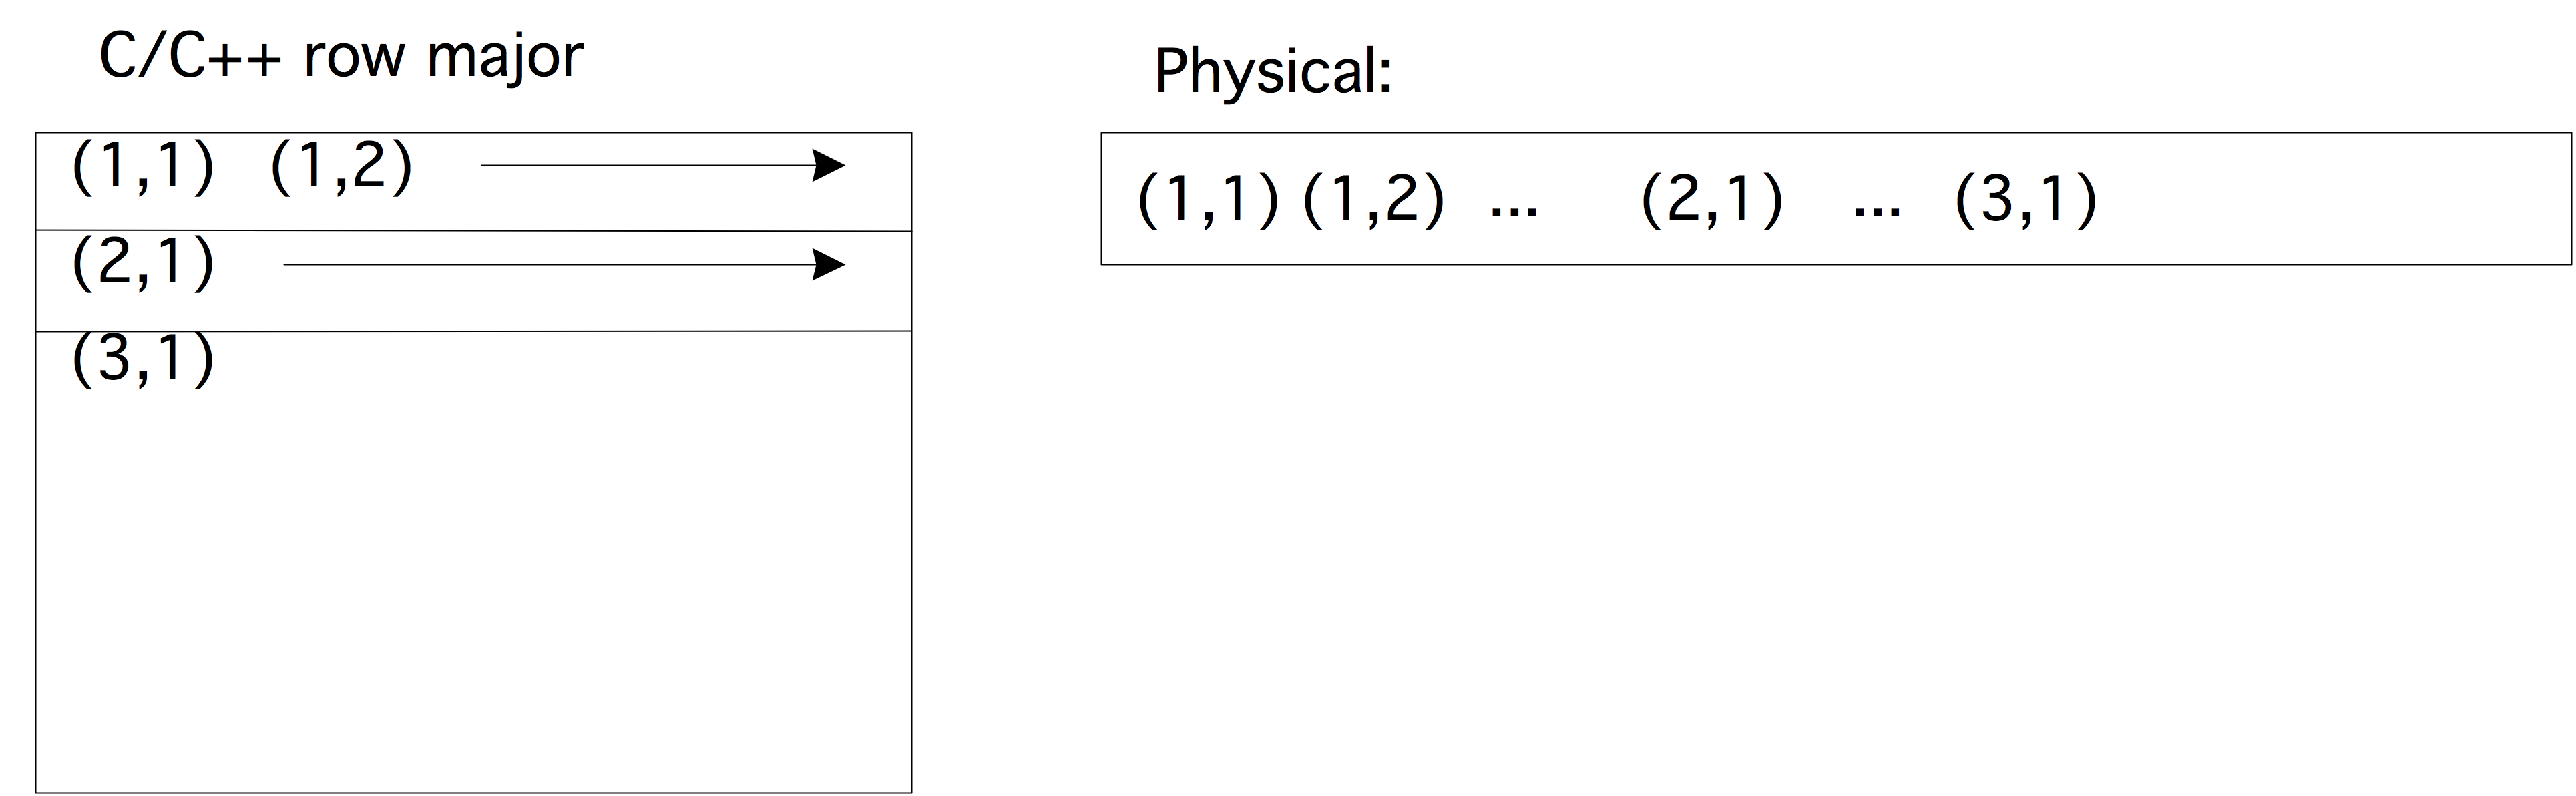
\includegraphics[scale=.1]{arrayc}

\Level 1 {Memory layout}

Puzzling aspects of arrays, such as which dimensions need to be
specified and which not in a function call, can be understood by
considering how arrays are stored in memory.
The question then is how a two-dimensional (or higher dimensional)
array is mapped to memory, which is linear.
\begin{itemize}
\item A one-dimensional array is stored in contiguous memory.
\item A two-dimensional array is also stored contiguously, with first
  the first row, then the second, et cetera.
\item Higher dimensional arrays continue this notion, with contiguous
  blocks of the highest so many dimensions.
\end{itemize}

As a result of this, indexing beyond the end of a row, brings you to the
start of the next row:
%
\verbatimsnippet{arraywrap}

We can now also understand how arrays are passed to functions:
\begin{itemize}
\item The only information passed to a function is the address of the
  first element of the array;
\item In order to be able to find location of the second row (and
  third, et cetera), the subprogram needs to know the length of each
  row.
\item In the higher dimensional case, the subprogram needs to know the
  size of all dimensions except for the first one.
\end{itemize}

\Level 0 {Exercises}

\begin{exercise}
  \label{ex:even-index}
  Given a vector of integers, write two loops;
  \begin{enumerate}
  \item One that sums all even elements, and
  \item one that sums all elements with even indices.
  \end{enumerate}
  Use the right type of loop.
\end{exercise}

\begin{exercise}
  Program \indexterm{bubble sort}: go through the array comparing
  successive pairs of elements, and swapping them if the second is
  smaller than the first. After you have gone through the array, the
  largest element is in the last location. Go through the array again,
  swapping elements, which puts the second largest element in the
  one-before-last location. Et cetera.
\end{exercise}

\begin{block}{Pascal's triangle}
  \label{sl:pascal-def}
  \small
  \indexterm{Pascal's triangle} contains binomial coefficients:
{\scriptsize
\begin{verbatim}
Row    1:                     1
Row    2:                   1   1
Row    3:                 1   2   1
Row    4:               1   3   3   1
Row    5:             1   4   6   4   1
Row    6:           1   5  10  10   5   1
Row    7:         1   6  15  20  15   6   1
Row    8:       1   7  21  35  35  21   7   1
Row    9:     1   8  28  56  70  56  28   8   1
Row   10:   1   9  36  84 126 126  84  36   9   1
\end{verbatim}
}
where \[ p_{rc} = \begin{pmatrix} r\\c \end{pmatrix} = \frac{r!}{c!(r-c)! }. \]
The coefficients can be computed from the recurrence
\[ p_{rc} = 
\begin{cases}
  1&c\equiv 1\vee c\equiv r\\
  p_{r-1,c-1}+p_{r-1,c}
\end{cases}
\]
(There are other formulas. Why are they less preferable?)
\end{block}

\begin{exercise}
  \label{ex:pascal-ex}
  \small
  \begin{itemize}
  \item 
    Write a class \n{pascal} so that \n{pascal(n)} is the object
    containing $n$~rows of the above coefficients. Write a method
    \n{get(i,j)} that returns the $(i,j)$ coefficient.
  \item
    Write a method \n{print} that prints the above display.
  \item First print out the whole pascal triangle; then:
  \item
    Write a method \n{print(int m)} that prints a star if the
    coefficient modulo~$m$ is nonzero, and a space otherwise.
\begin{verbatim}
          *
         * *
        *   *
       * * * *
      *       *
     * *     * *
    *   *   *   *
   * * * * * * * *
  *               *
 * *             * *
\end{verbatim}
  \end{itemize}
\end{exercise}
\begin{block}{Exercise continued}
  \label{sl:pascal-ex-contd}
  \begin{itemize}
  \item
    The object needs to have an array internally. The easiest solution
    is to make an array of size $n\times n$.
  \item Your program should accept:
    \begin{enumerate}
    \item
      an integer for the size
    \item any number of integers for the modulo; if this is zero, stop,
      otherwise print stars as described above.
    \end{enumerate}
  \end{itemize}
\end{block}


\begin{exercise}
  \label{ex:pascal-ey}
  Extend the Pascal exercise:\\
  Optimize your code to use
  precisely enough space for the coefficients.
\end{exercise}

\begin{exercise}
  A knight on the chess board moves by going two steps horizontally or
  vertically, and one step either way in the orthogonal
  direction. Given a starting position, find a sequence of moves that
  brings a knight back to its starting position. Are there starting
  positions for which such a cycle doesn't exist?
\end{exercise}

\begin{exercise}
  From the `Keeping it REAL' book, exercise 3.6 about Markov chains.
\end{exercise}

\begin{figure}[ht]
  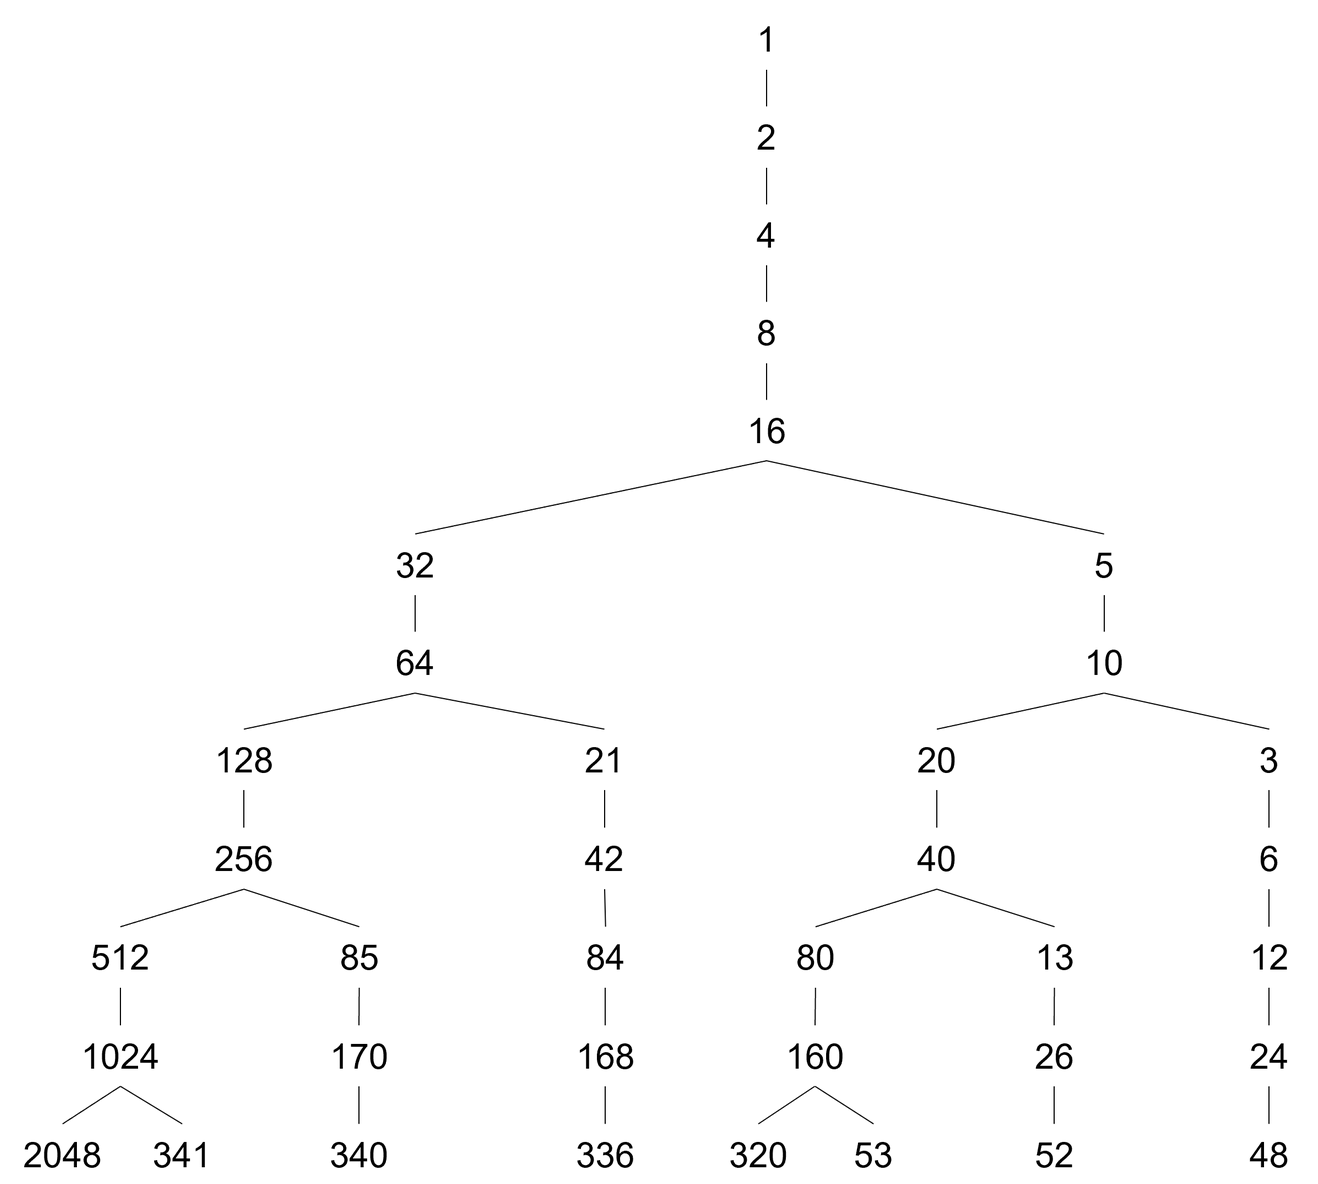
\includegraphics[scale=.5]{collatz-tree}
  \caption{The `Collatz tree'}
  \label{fig:collatz-tree}
\end{figure}

\begin{exercise}
  Revisit exercise~\ref{ex:collatz},
  and generate the `Collatz tree' (figure~\ref{fig:collatz-tree}):
  at level $n$ (one-based counting)
  are the numbers that in $n-1$ steps converge to~1.

  Read in a number $n$ and print the first $n$ rows,
  each row on a new line, with the numbers separated by spaces.
\end{exercise}

\ifIncludeAnswers
\else
\endinput
\fi

\Level 0 {Homework discussions}

\Level 1 {Pascal}
\label{sec:pascal-discussion}

\begin{multicols}{2}
  \scriptsize
  \lstset{basicstyle=scriptsize}
  \input pascal_discussion
  \lstset{basicstyle=footnotesize}
\end{multicols}
